\section{From Chords to Shadows: The Rise of Islamic Trigonometry}


\subsection{A Complete Set of Trigonometric Functions}

Ptolemy’s *Almagest* laid the geometric groundwork for astronomy, using chords and circle theorems to describe celestial motion. But centuries later, Islamic mathematicians took that foundation and transformed it — turning geometry into a full-fledged **computational language of the heavens**.

One of the most pivotal figures in this transformation was \textbf{Al-Battani} (c.~858–929 CE), a Syrian astronomer who revised and refined Ptolemy’s models with a revolutionary insight: instead of using the Greek \textit{chord} function, he adopted the Indian concept of the \textbf{sine}. From this change blossomed an entirely new system — what we now call **trigonometry**.

Islamic mathematicians were the first to treat all six trigonometric functions — sine, cosine, tangent, cotangent, secant, and cosecant — as independent mathematical entities. Each was defined geometrically, not as a ratio between abstract variables, but as literal line segments within a right triangle or a circle.

\begin{center}
\renewcommand{\arraystretch}{1.4}
\begin{tabular}{|c|c|p{6cm}|}
\hline
\textbf{Function} & \textbf{Arabic Name} & \textbf{Conceptual Basis} \\
\hline
\( \sin \theta \) & \textit{Jyb} (جيب) & Half-chord in a circle; directly replaced the Greek chord function \\
\( \cos \theta \) & \textit{Zill} (ظل) & “Shadow” of the complementary angle; visualized geometrically \\
\( \tan \theta \) & \textit{Zill Mustawi} (ظل مستوي) & “Straight shadow”; defined as a line touching the circle tangent to the radius \\
\( \cot \theta \) & \textit{Zill Muʿākis} (ظل معكوس) & “Reversed shadow” \\
\( \sec \theta \) & \textit{Qāṭiʿ} (قاطع) & “Cutter”; length of a secant from center to tangent \\
\( \csc \theta \) & \textit{Munqāṭiʿ} (منقاطع) & “Cut-off”; reciprocal of sine, defined as line segment \\
\hline
\end{tabular}
\end{center}

Unlike later symbolic definitions, these functions were treated as measurable quantities. A triangle wasn’t an abstraction — it was an instrument.

\subsection{Precision Tables and Sexagesimal Computation}

Astronomers like Al-Battani and Al-Tusi compiled detailed trigonometric tables in degrees and sexagesimal subdivisions (base-60), a practice inherited from Babylonian astronomy.

\begin{center}
\begin{tabular}{|c|c|c|}
\hline
\textbf{Angle (°)} & \textbf{Sine (base 60)} & \textbf{Tangent (base 60)} \\
\hline
30° & 0;30,00 & 0;57,17 \\
45° & 0;42,25 & 1;00,00 \\
60° & 0;51,57 & 1;43,14 \\
\hline
\end{tabular}
\end{center}

For example, \( 0;30,00 \) means \( \frac{1}{2} \), and \( 0;42,25 \approx \frac{\sqrt{2}}{2} \). Interpolation between values was performed geometrically and algorithmically.

\subsection{Spherical Trigonometry and the Shape of the Sky}

Islamic scholars did not limit themselves to planar triangles. They extended trigonometric reasoning to the celestial sphere — essential for:

\begin{itemize}
    \item Predicting the positions of stars and planets
    \item Calculating solar and lunar altitudes
    \item Determining the visibility of the new crescent moon
\end{itemize}

They formalized results like the spherical law of cosines:

\[
\cos c = \cos a \cos b + \sin a \sin b \cos C
\]

This identity — used to solve triangles on a sphere — predates its rediscovery in Europe by several centuries.

\subsection{Instruments of Trigonometric Astronomy}

The innovations were not just theoretical. Instruments like the \textbf{astrolabe} and the \textbf{quadrant} were physical embodiments of trigonometric insight.

\begin{itemize}
    \item Astrolabes used sine-based calculations to measure altitude and time.
    \item Quadrants had curves etched directly onto them for sine and cosine values.
\end{itemize}

These devices made trigonometry tactile.

\subsection{Applications: Astronomy, Religion, and Earthly Orientation}

\paragraph{Spherical Astronomy:} Trigonometry was essential for modeling the night sky. Given a star’s declination \( \delta \), the observer’s latitude \( \phi \), and the hour angle \( H \), astronomers used:

\[
\sin h = \sin \phi \sin \delta + \cos \phi \cos \delta \cos H
\]

This equation — known today as the altitude formula — let astronomers compute the star’s position on the horizon at any time.

\paragraph{Qibla and Prayer Times:} Islamic astronomers also used trigonometry to determine:

\begin{itemize}
    \item The \textbf{qibla} (direction to Mecca)
    \item The times for prayer, based on solar altitude and position
\end{itemize}

These required solving spherical triangles formed by the zenith, Mecca, and the celestial pole.

\paragraph{Planetary Models:} Building on Ptolemaic systems, astronomers like Al-Tusi developed more accurate planetary models, including the **Tusi couple** — a pair of rotating circles that produced linear motion, used to explain oscillating planetary paths. This was a geometric mechanism rooted in trigonometric understanding and would anticipate aspects of Kepler's work centuries later.

\paragraph{Observatories:} At places like Maragha (13th century) and Samarkand (15th century), astronomers like **Nasir al-Din al-Tusi** and **Ulugh Beg** built enormous observational tools. These observatories featured walls marked with sine scales and sighting tubes aligned using precise angular measurements.

\subsection{Legacy}

Islamic trigonometry transformed a geometric toolkit into a scientific method. It shifted astronomy from approximation to calculation — not by abandoning Ptolemy, but by completing him.

\medskip

\begin{tcolorbox}[colback=gray!5!white, colframe=black, title=\textbf{TL;DR: When Trigonometry Became a Science}, fonttitle=\bfseries, arc=1.5mm, boxrule=0.4pt]
Islamic mathematicians and astronomers were the first to fully formalize all six trigonometric functions as geometric entities. They developed sine-based models that replaced Greek chords, constructed interpolation tables in sexagesimal form, and applied these tools to planetary prediction, spherical astronomy, religious timekeeping, and precision instrumentation.

They didn’t just use trigonometry — they \textbf{turned it into a discipline}.
\end{tcolorbox}

\begin{figure}[H]
    \centering
    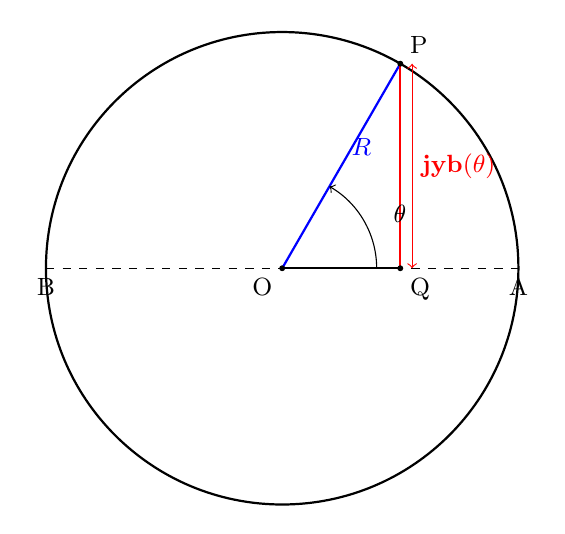
\begin{tikzpicture}[scale=3, every node/.style={font=\small}]
    
      % Draw unit circle
      \draw[thick] (0,0) circle(1);
    
      % Radius at angle theta
      \draw[thick, blue] (0,0) -- (60:1) node[pos=0.5, above right] {$R$};
    
      % Horizontal diameter
      \draw[dashed] (-1,0) -- (1,0);
    
      % Project vertical to x-axis (sine)
      \draw[dotted] (60:1) -- (60:1 |- 0,0);
    
      % Mark right triangle components
      \draw[thick, red] (60:1 |- 0,0) -- (60:1);
      \draw[thick] (0,0) -- (60:1 |- 0,0);
    
      % Label sine segment
      \draw[<->, red] (60:1 |- 0,0) + (0.05, 0) -- +(0.05, {sin(60)}) node[midway, right] {\textbf{jyb$(\theta)$}};
    
      % Angle arc
      \draw[->] (0.4,0) arc[start angle=0, end angle=60, radius=0.4];
      \node at (25:0.55) {$\theta$};
    
      % Points
      \filldraw[black] (0,0) circle(0.01) node[below left] {O};
      \filldraw[black] (60:1) circle(0.01) node[above right] {P};
      \filldraw[black] (60:1 |- 0,0) circle(0.01) node[below right] {Q};
    
      % Optional helper labels
      \node[below] at (1,0) {A};
      \node[below] at (-1,0) {B};
    
    \end{tikzpicture}
    \caption{Geometric definition of sine in Islamic trigonometry: the line segment \textbf{jyb$(\theta)$} is the vertical from the circle point \( P \) to the diameter — half the chord of \( 2\theta \).}
\end{figure}


\begin{tcolorbox}[colback=gray!5!white, colframe=black, title=\textbf{Historical Sidebar: The Islamic Lunar Calendar}, fonttitle=\bfseries, arc=1.5mm, boxrule=0.4pt]

    The \textbf{Islamic calendar}, also known as the \textit{Hijri calendar}, is a purely \textbf{lunar calendar} — each month begins with the first visible sighting of the new crescent moon (\textit{hilal}) after conjunction.
    
    Unlike solar calendars, the Islamic calendar is not synchronized with the seasons. Each year is approximately 354 days long, drifting through the solar year over a 33-year cycle. This means that Ramadan, for instance, occurs in all seasons over time.
    
    \medskip
    
    \textbf{Why this mattered for astronomy:}
    
    Islamic scholars had to accurately predict the \textit{visibility} of the new moon — a nontrivial task. It depends on:
    
    \begin{itemize}
        \item The Moon's age after conjunction,
        \item Its angular distance from the Sun,
        \item Its altitude at sunset,
        \item The observer's location on Earth.
    \end{itemize}
    
    This made lunar visibility a problem in \textbf{spherical astronomy}, not just geometry. Trigonometric calculations — often involving the spherical law of cosines — were essential for determining if the crescent could be seen on a given evening.
    
    \medskip
    
    Religious scholars (the \textit{muwaqqitūn}, or timekeepers) worked alongside astronomers to provide tables and instruments to estimate the crescent’s appearance. Some Islamic observatories even included horizon-viewing platforms specifically designed for this purpose.
    
    \medskip
    
    \textbf{Legacy:} The need to observe lunar phases with high precision helped drive the development of trigonometry, observational instruments, and spherical coordinate systems. Even today, debates around \textit{hilal} sighting blend astronomy, jurisprudence, and tradition — a lasting legacy of this centuries-old scientific-religious synthesis.
    
\end{tcolorbox}


\begin{figure}[H]
    \centering
    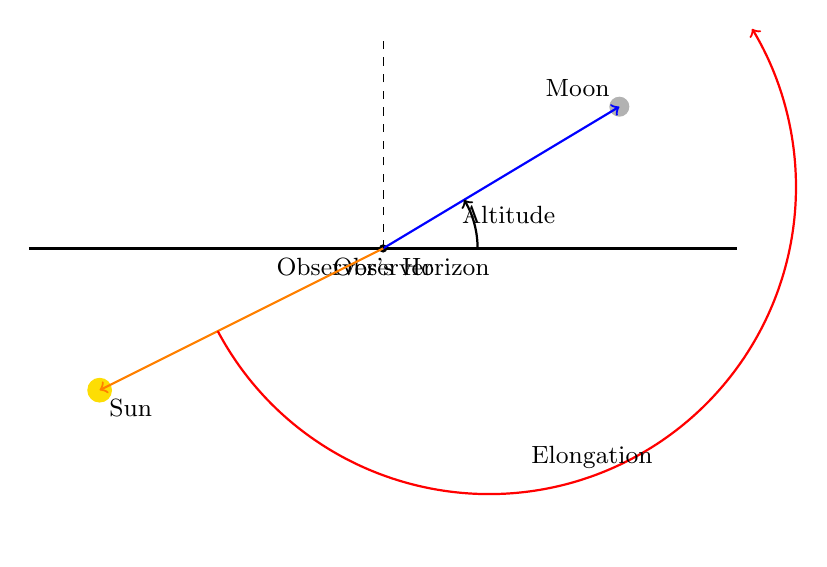
\begin{tikzpicture}[scale=3, every node/.style={font=\small}]
    
      % Ground/horizon line
      \draw[thick] (-1.5,0) -- (1.5,0);
      \node[below] at (0,0) {Observer's Horizon};
    
      % Observer
      \filldraw[black] (0,0) circle (0.015) node[below] {Observer};
    
      % Sun below horizon
      \filldraw[yellow!80!orange] (-1.2,-0.6) circle (0.05);
      \node[below right] at (-1.2,-0.6) {Sun};
    
      % Moon above horizon
      \filldraw[gray!60] (1.0,0.6) circle (0.04);
      \node[above left] at (1.0,0.6) {Moon};
    
      % Line of sight to Moon
      \draw[thick, ->, blue] (0,0) -- (1.0,0.6);
    
      % Line to Sun (below horizon)
      \draw[thick, ->, orange] (0,0) -- (-1.2,-0.6);
    
      % Altitude angle
      \draw[->, thick] (0.4,0) arc[start angle=0, end angle=31, radius=0.4];
      \node at (15:0.55) {Altitude};
    
      % Elongation angle (angle between Sun and Moon)
      \draw[->, thick, red] (-0.7,-0.35) arc[start angle=-152, end angle=31, radius=1.3];
      \node at (-45:1.25) {Elongation};
    
      % Horizon label
      \draw[dashed] (0,0) -- (0,0.9);
    
    \end{tikzpicture}
    \caption{Crescent visibility geometry: The Moon’s visibility depends on its altitude and elongation angle (Sun–Moon separation). Both angles were computed using spherical trigonometry.}
\end{figure}


\begin{figure}[H]
    \centering
    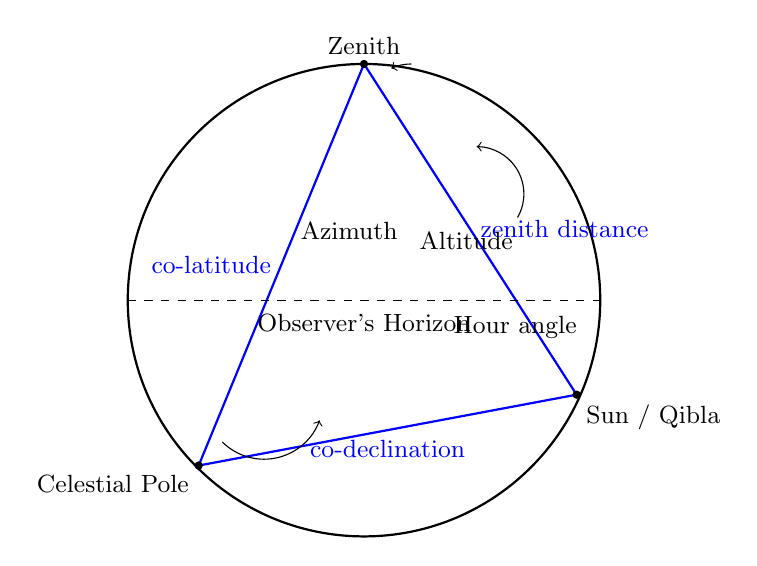
\begin{tikzpicture}[scale=3, every node/.style={font=\small}]
    
    % Sphere base
    \draw[thick] (0,0) circle(1);
    
    % Points
    \coordinate (Z) at (0,1);  % Zenith
    \coordinate (P) at (-0.7,-0.7); % Celestial Pole (North)
    \coordinate (S) at (0.9,-0.4); % Celestial Object (Sun or Qibla)
    
    % Triangle sides
    \draw[thick, blue] (Z) -- (P) node[midway, left] {co-latitude};
    \draw[thick, blue] (P) -- (S) node[midway, below] {co-declination};
    \draw[thick, blue] (S) -- (Z) node[midway, right] {zenith distance};
    
    % Mark points
    \filldraw[black] (Z) circle (0.015) node[above] {Zenith};
    \filldraw[black] (P) circle (0.015) node[below left] {Celestial Pole};
    \filldraw[black] (S) circle (0.015) node[below right] {Sun / Qibla};
    
    % Angles
    \draw[->] (0.2,1) arc[start angle=90, end angle=115, radius=0.2];
    \node at (102:0.3) {Azimuth};
    
    \draw[->] (-0.6,-0.6) arc[start angle=225, end angle=340, radius=0.25];
    \node at (-10:0.65) {Hour angle};
    
    \draw[->] (0.65,0.35) arc[start angle=330, end angle=450, radius=0.2];
    \node at (30:0.5) {Altitude};
    
    % Horizon line
    \draw[dashed] (-1,0) -- (1,0);
    \node[below] at (0,-0.02) {Observer’s Horizon};
    
    \end{tikzpicture}
    \caption{Spherical triangle used in Islamic astronomy: Between the Zenith, Celestial Pole, and a celestial object (e.g., Sun or Qibla). Angular geometry allowed computation of Qibla direction, prayer times, and celestial events.}
\end{figure}


\begin{tcolorbox}[colback=gray!5!white, colframe=black, title=\textbf{Historical Sidebar: When Prayer Became a Global Problem}, fonttitle=\bfseries, arc=1.5mm, boxrule=0.4pt]

    In the early centuries of Islam, prayer times were a local matter. The five daily prayers — anchored to the position of the Sun — could be estimated by observing shadows, sunrise, and sunset. In Mecca and Medina, this worked with simplicity and reliability.
    
    But as Islam expanded into Persia, Central Asia, North Africa, and beyond, a problem emerged: \textbf{solar behavior varies dramatically with latitude}. Near the equator, days and nights are relatively stable. But farther north or south, shadow lengths change unevenly, and daylight hours can stretch or vanish with the seasons.
    
    \medskip
    
    In places like Damascus, Córdoba, or Samarkand, determining the time for \textit{Fajr} (dawn), \textit{Asr} (afternoon), or \textit{Isha} (night) became a nontrivial mathematical task — especially in seasons when the Sun barely dipped below the horizon.
    
    \medskip
    
    This challenge gave rise to a new scientific vocation: the \textbf{muwaqqit} — the mosque timekeeper — who used instruments and astronomy to calculate proper times for worship.
    
    \medskip
    
    Enter \textbf{Al-Battani} (c.~858–929), one of the most precise astronomers of the Islamic Golden Age. His \textit{Zīj} (astronomical tables) included detailed values for:
    \begin{itemize}
      \item The Sun’s \textbf{declination} (its latitude on the celestial sphere),
      \item Its \textbf{altitude} above the horizon at given times and dates,
      \item The equations needed to convert this data into prayer times.
    \end{itemize}
    
    \medskip
    
    By tabulating these values, Al-Battani made it possible for timekeepers across the Islamic world — from Cairo to Córdoba — to calculate accurate prayer times using spherical trigonometry rather than guesswork.
    
    \medskip
    
    \textbf{Prayer had become global, and astronomy rose to meet it.}
    
\end{tcolorbox}








\section{Regiomontanus and the Birth of Trigonometry as a Discipline}

By the 15th century, European mathematics was beginning to reawaken — and one of its clearest signs was the appearance of a book that, for the first time, treated trigonometry as an independent mathematical subject.

That book was \textit{De Triangulis Omnimodis} (On Triangles of Every Kind), written around 1464 by the German mathematician \textbf{Johann Müller}, better known as \textbf{Regiomontanus}.

\medskip

Unlike earlier astronomers who embedded trigonometry within celestial models or tables, Regiomontanus organized it as a coherent mathematical system. His work drew heavily from Islamic sources — particularly the chord-based trigonometry of Al-Battani and Al-Tusi — but restructured them using the evolving notational tools of Renaissance Europe.

\medskip

\textbf{What made \textit{On Triangles} groundbreaking?}
\begin{itemize}
  \item It was the first European text to treat \textbf{trigonometry as a branch of mathematics} — not just a tool for astronomy.
  \item It gave explicit attention to both \textbf{plane} and \textbf{spherical triangles}, covering the general rules for solving them.
  \item It included clear statements of what we now call the \textbf{Law of Sines} and \textbf{Law of Cosines}.
  \item It synthesized Greek geometry and Islamic trigonometric techniques using Latin terminology and notation.
\end{itemize}

\medskip

Regiomontanus was also a practicing astronomer and instrument-maker, and his goal was practical as well as theoretical: to provide accurate methods for celestial navigation, eclipse prediction, and positional astronomy — all through a unified geometric lens.

\medskip

\textbf{Legacy:} Though his book would not be printed until 1533 (after his death), \textit{On Triangles} became the template for trigonometry in the Latin West — a text that signaled the transition from geometry as pure form to geometry as computational science.

\begin{tcolorbox}[colback=gray!5!white, colframe=black, title=\textbf{TL;DR: The First Book of Trigonometry}, fonttitle=\bfseries, arc=1.5mm, boxrule=0.4pt]
\textit{De Triangulis Omnimodis} by Regiomontanus (1464) was the first European work to define trigonometry as a standalone discipline.  
It unified the spherical methods of Islamic astronomy with classical geometry, and turned trigonometry into a proper branch of mathematics — not just a set of tables.
\end{tcolorbox}




